\section{Supplemental Results}\label{sup}
\begin{table}[h]
  \caption{Notation}
  \label{tab:notation}
  \centering
  \begin{tabular}{cl}
  \toprule
    Symbol   & Definition                                        \\
  \midrule
  $\lambda$  & Rate of infection per susceptible person          \\
  $\lambda'$ & Rate of transmission per infectious person        \\
  $\Lambda$  & Rate of all new infections in the population      \\
   $\beta$   & Probability of transmission per contact (sex act) \\
     $A$     & Total contacts per partnership                    \\
     $B$     & Probability of transmission per partnership       \\
     $Q$     & Rate of partnership formation                     \\
     $F$     & Rate (frequency) of contacts per partnership      \\
     $C$     & Number of concurrent partnerships                 \\
     $R$     & Relative probability of transmission per contact  \\
   $\alpha$  & Proportion of contacts per partnership affected   \\
  $\Delta_t$ & Time period                                       \\
  \bottomrule
\end{tabular}
\end{table}
%\subsection{Binomial Adjustment: Examples of Bias}\label{sup.bin} % TODO
\begin{figure}[h]
  \centerline{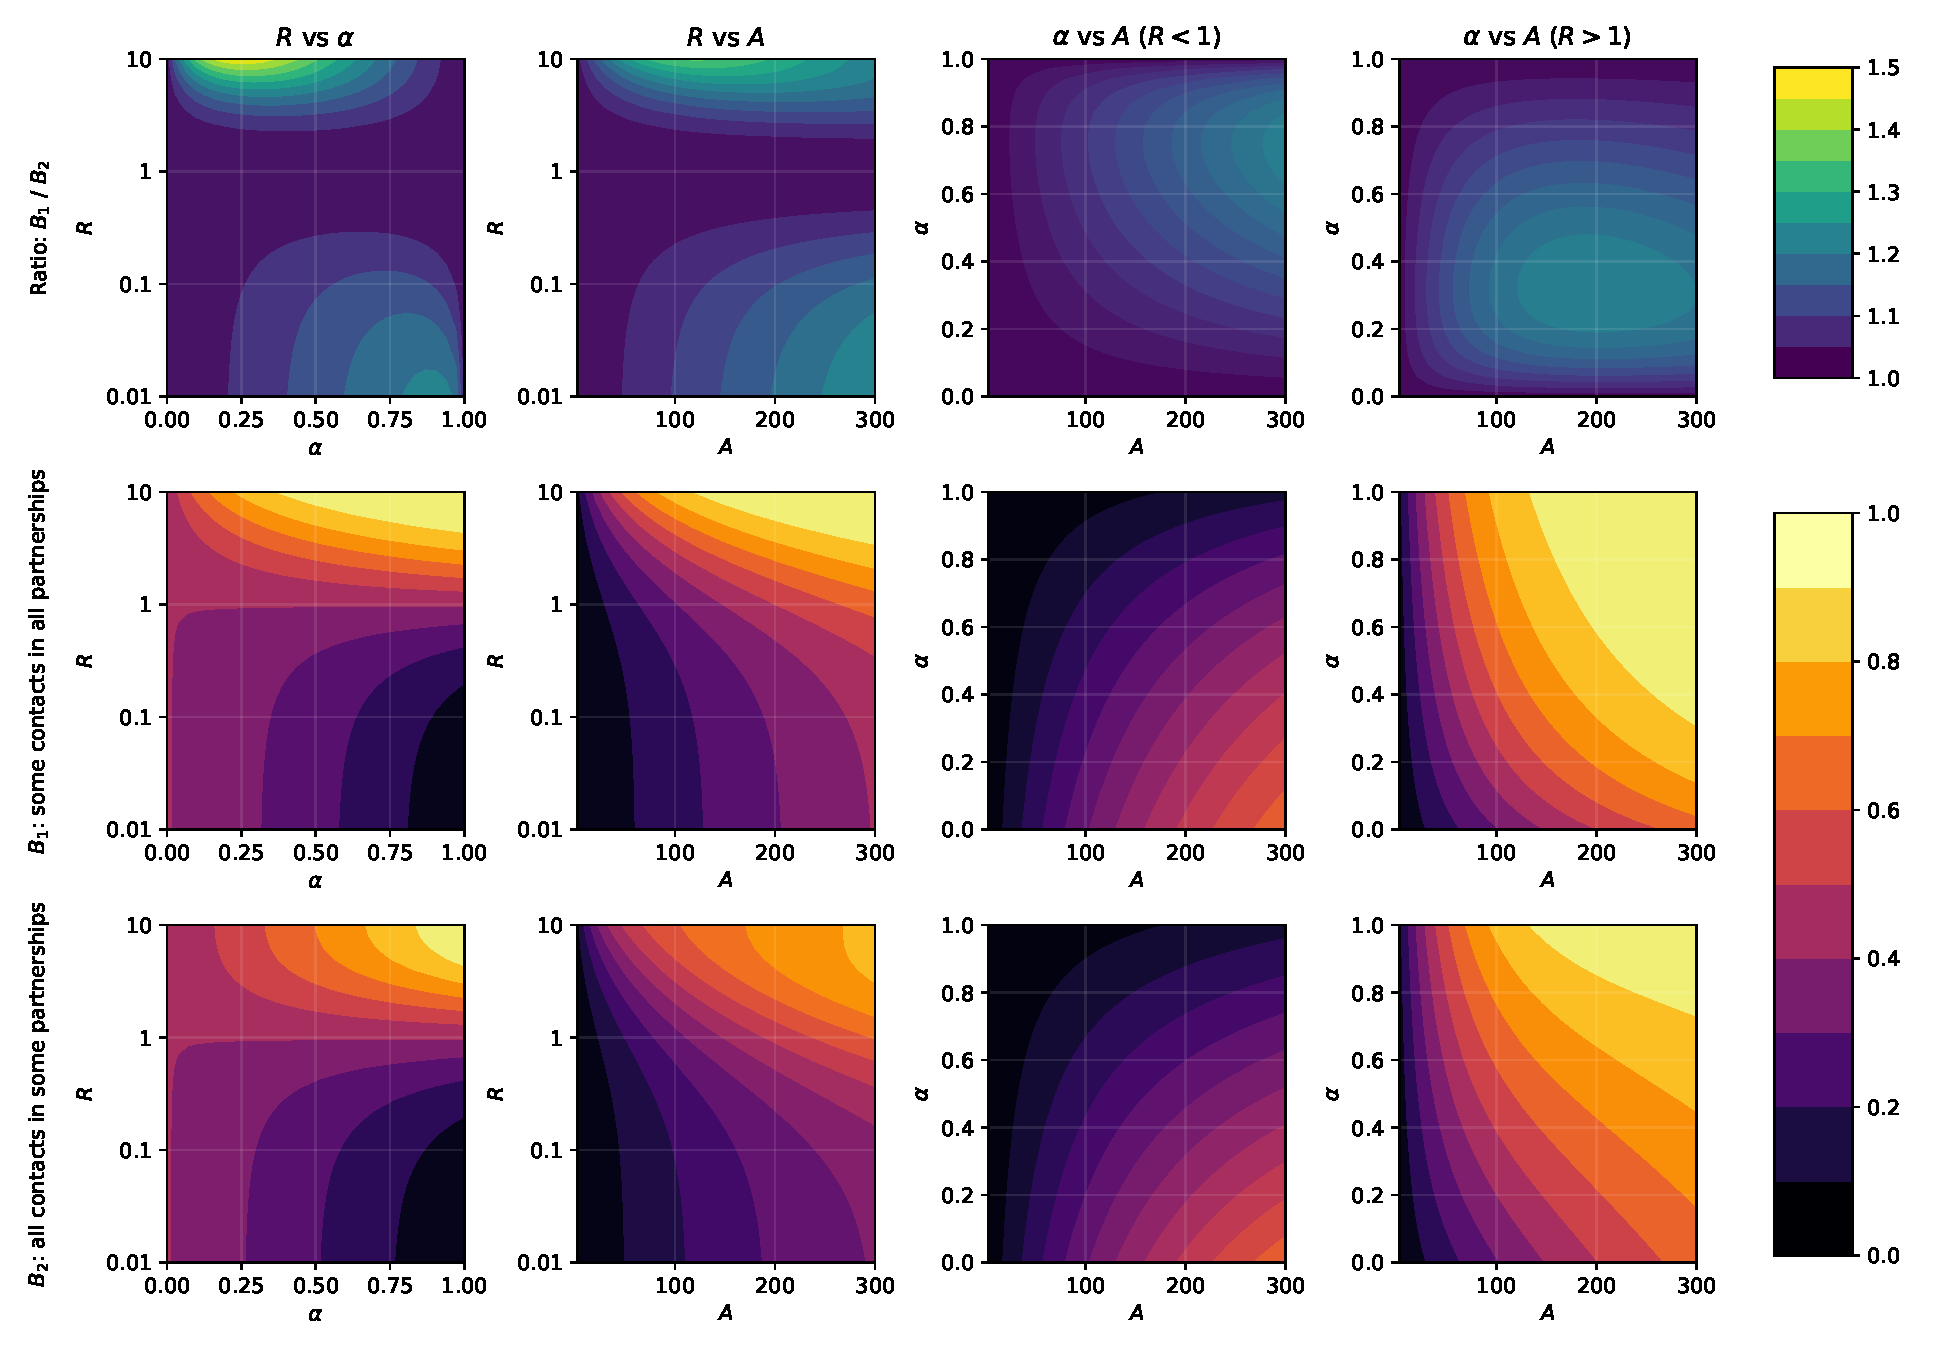
\includegraphics[width=\widefig]{B.mod.vs}}
  \caption{Per-partnership probability of transmission $B$,
    in the presence of a transmission modifier $R$, calculated assuming either:
    $B_1$: $\alpha$ proportion of contacts in all partnerships modified; or
    $B_2$: all contacts in $\alpha$ proportion of partnerships modified.
    We observe $B_1 \ge B_2$.}
  \label{fig:B.mod.sens}
  \floatfoot
  $\beta = 0.34\%$ throughout \cite{Boily2009}.
  For $R$ vs $\alpha$, $A = 152$;
  for $R$ vs $A$, $\alpha = 0.5$;
  for $\alpha$ vs $A$, $(R<1) = 0.1$, $(R>1) = 5$.
  For $0.1 < R < 3$, the ratio $B_1 / B_2 \approx 1$.
  When $R < 1$, then $B_1 / B_2$ is maximized with $A \rightarrow \infty$ and $0.5 < \alpha < 1$.
  When $R > 1$, then $B_1 / B_2$ is maximized with $1 < A < \infty$ and $0 < \alpha < 0.5$.
\end{figure}
\begin{figure}[h]
  \centerline{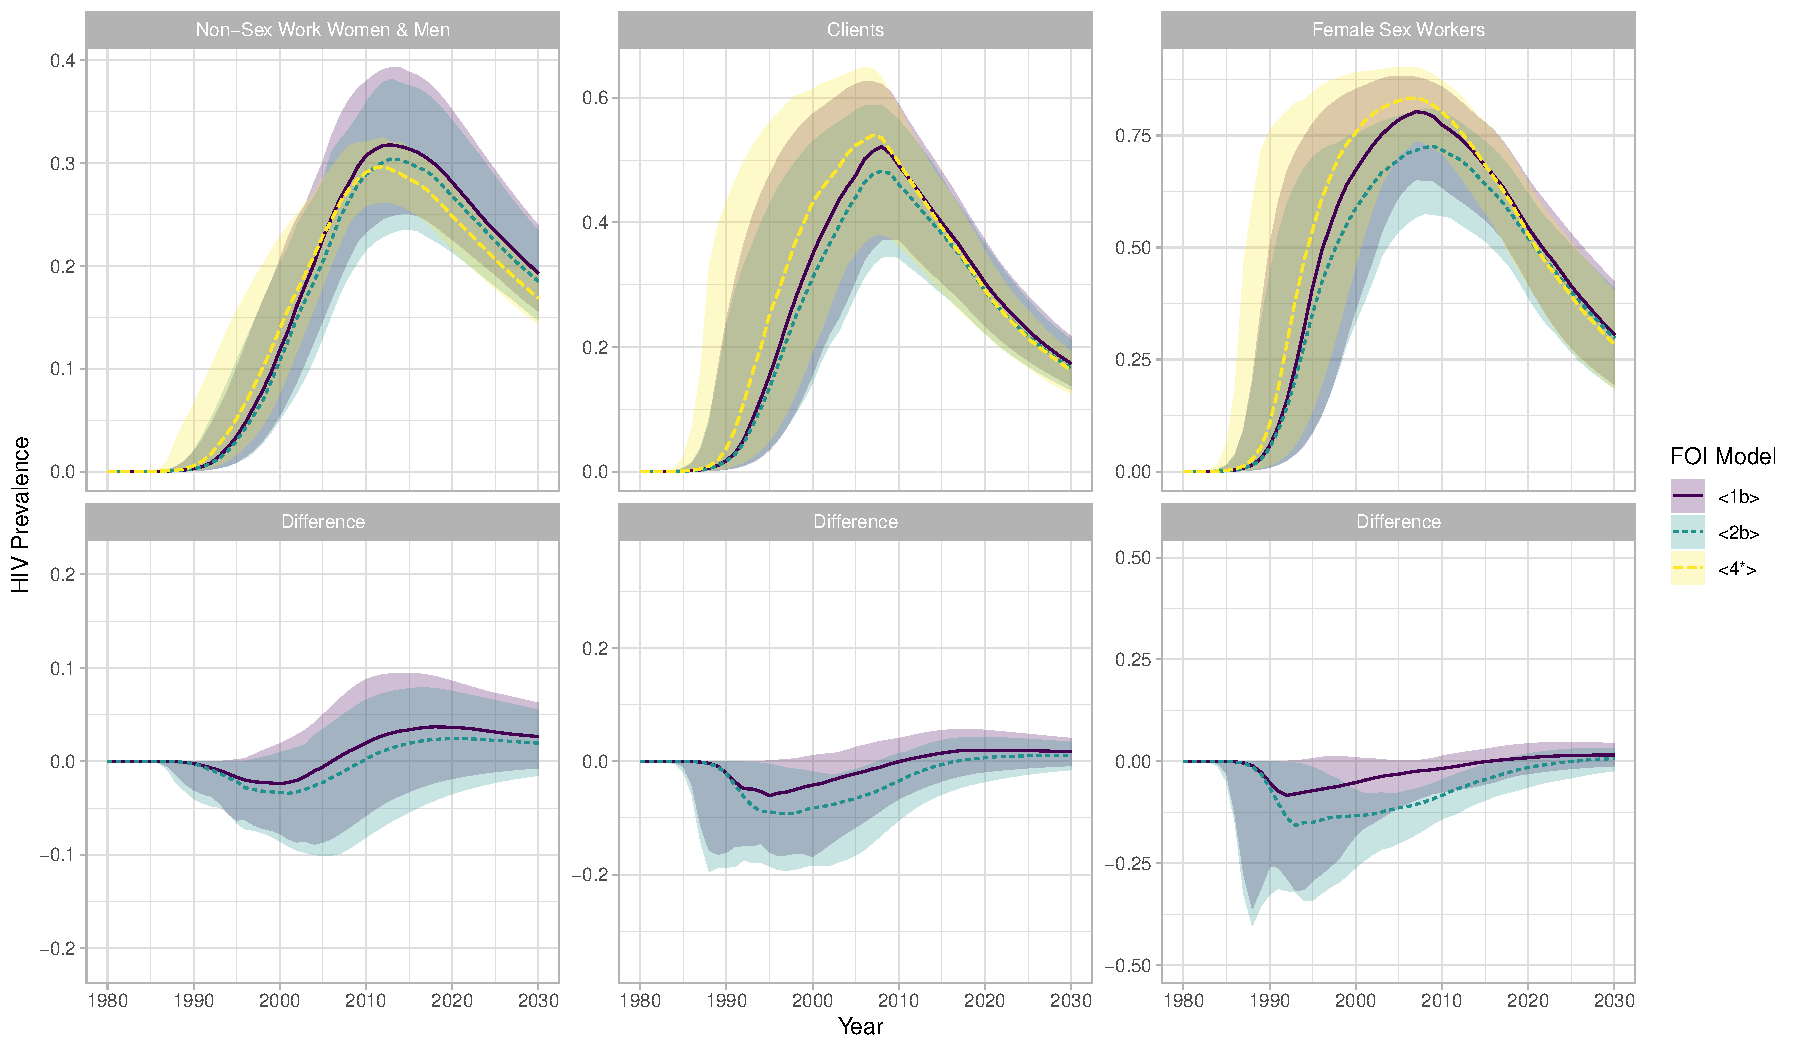
\includegraphics[width=\widefig]{foi.ep.prevalence}}
  \caption{Comparison of modelled prevalence under force of infection models
    \case{1a}, \case{1b}, \case{2b}, and \case{4*} with equal parameters}
  \label{fig:ep.prev}
  \floatfoot
  Model names:
  \case{1a} binomial per-partnership;
  \case{1b} binomial per-partnership-year;
  \case{2b} binomial per-year;
  \case{4*} partnership exclusion (proposed).
  Parameter values taken from the \case{4*} model fit with highest likelihood;
  for \case {1a}: $Q_{ijk} = C_{ijk} / \delta_k$, $A_{k} = F_{k} \delta_k$;
  for \case{1b} and \case{2b}: $Q_{ijk} = C_{ijk}$, $A_{k} = F_{k}$.
  Lines show median values and transparent ribbons show 90\% confidence intervals
  from top 1000 of 100,000 \case{4*} model fits.
\end{figure}
\begin{figure}[h]
  \begin{subfigure}{\linewidth}
    \centerline{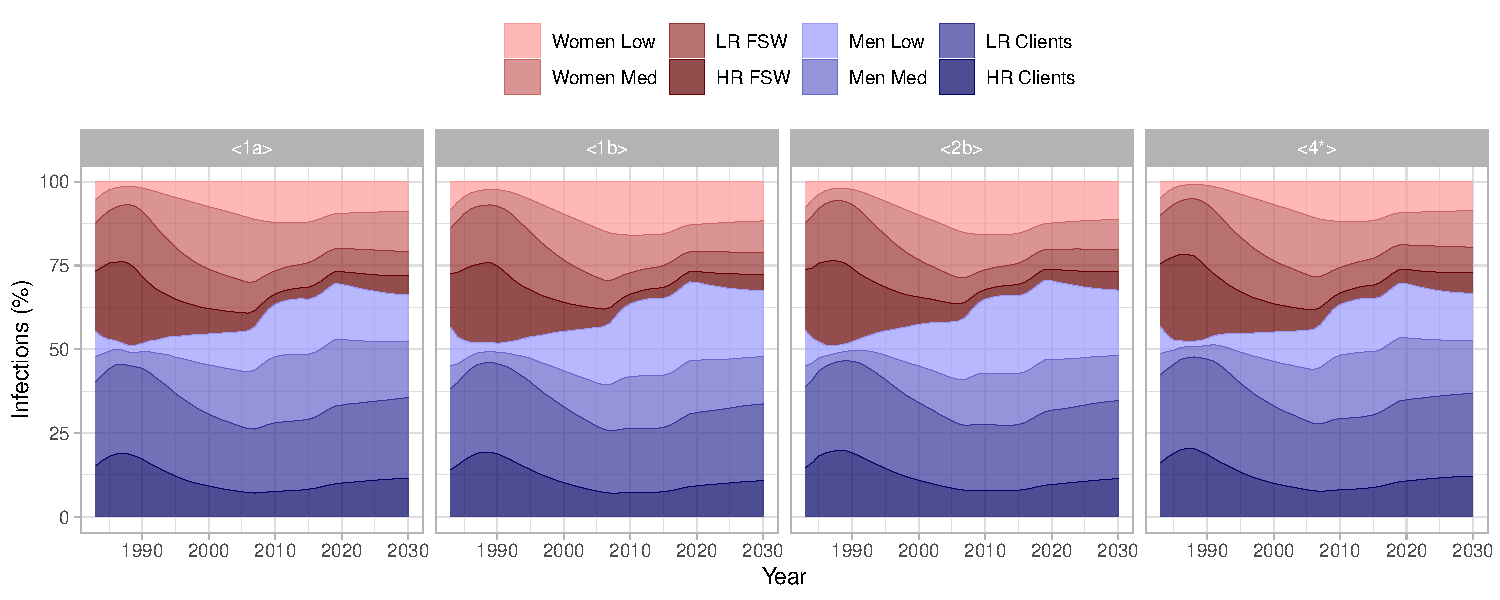
\includegraphics[width=\widefig]{inf-foi-from-rel}}
    \caption{From whom (transmitted)}
    \label{fig:inf.from}
  \end{subfigure}
  \begin{subfigure}{\linewidth}
    \centerline{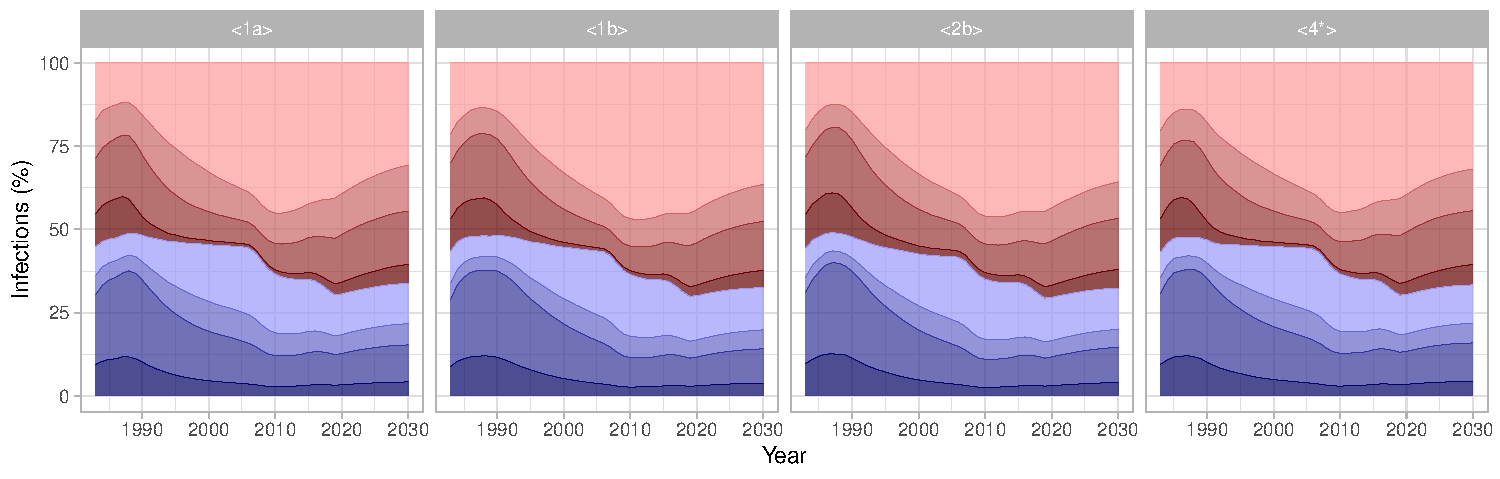
\includegraphics[width=\widefig]{inf-foi-to-rel}}
    \caption{To whom (acquired)}
    \label{fig:inf.to}
  \end{subfigure}
  \caption{Comparison of the distribution of yearly infections
    by transmitting and acquiring risk groups
    under calibrated force of infection models \case{1a}, \case{1b}, \case{2b}, and \case{4*}}
  \label{fig:inf.frto}
  \floatfoot
  FOI Model names:
  \case{1a} binomial per-partnership;
  \case{1b} binomial per-partnership-year;
  \case{2b} binomial per-year;
  \case{4*} partnership exclusion (proposed).
  Parameters were re-calibrated for each FOI model,
  and infections reflect the median value from
  the top 1000 of 100,000 model fits in each case.
  Risk groups definitions:
  Low: 0-1 partners in past 12 months (p12m);
  Med: 2+ partners p12m but no sex work;
  FSW: female sex workers;
  Clients: of FSW;
  LR / HR: lower risk (80\%) / higher risk (20\%).
\end{figure}
\begin{figure}[h]
  \centerline{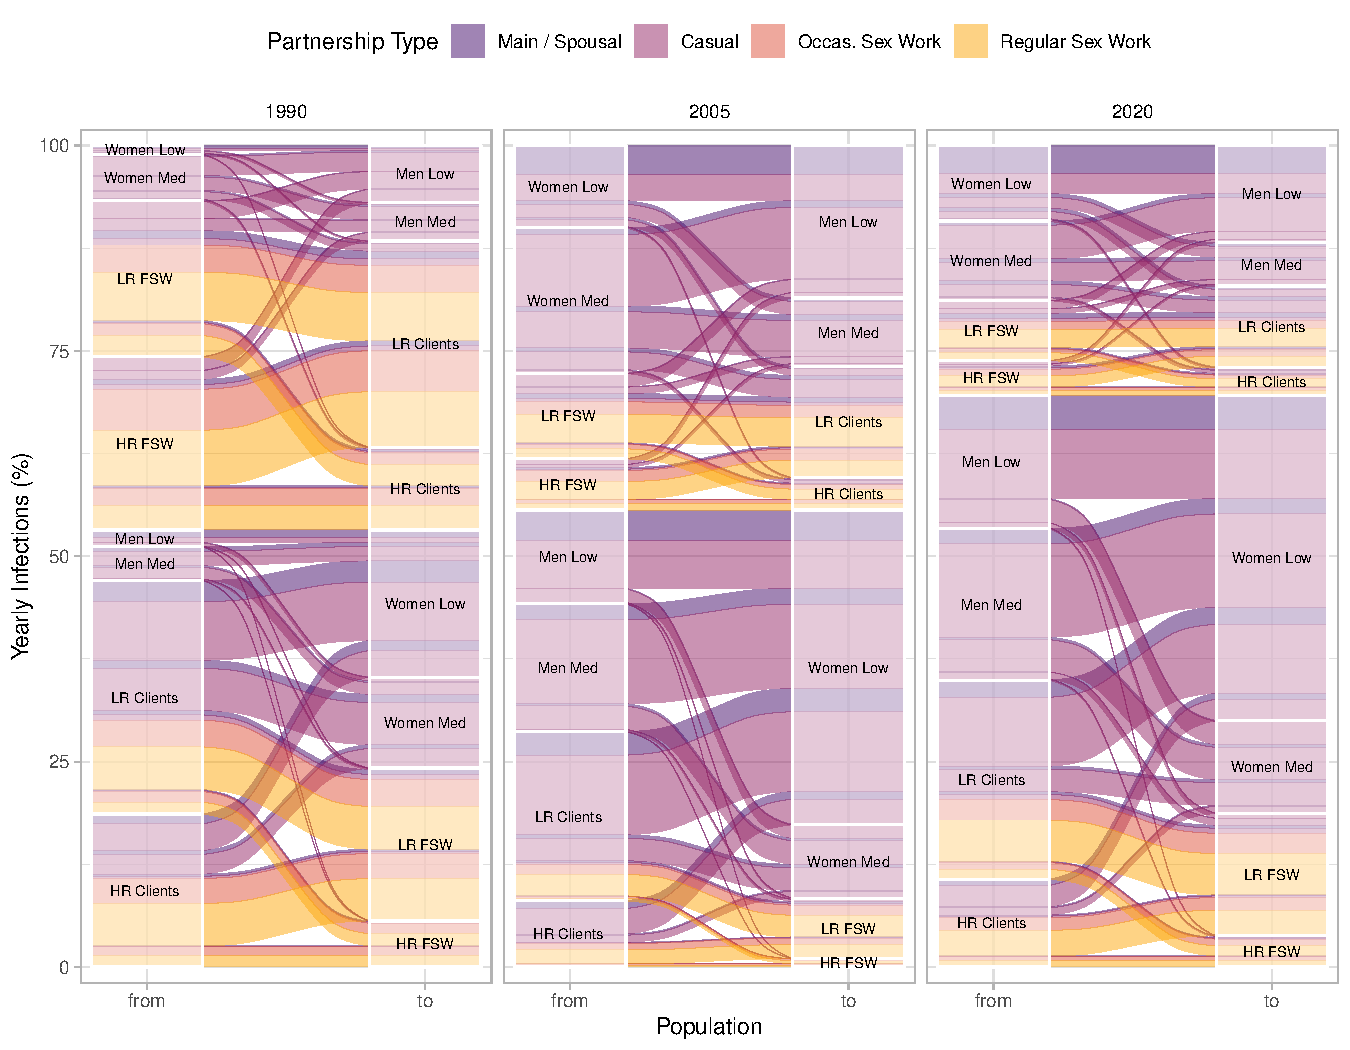
\includegraphics[width=\widefig]{inf-base-alluvial-3}}
  \caption{Distribution of yearly infections
    by partnership type and transmitting / acquiring risk groups
    under calibrated model \case{4*} in 1990, 2005, and 2020}
  \label{fig:inf.alluvial}
  \floatfoot
  Infections reflect the median value from
  the top 1000 of 100,000 model \case{4*} fits.
  Risk groups definitions:
  Low: 0-1 partners in past 12 months (p12m);
  Med: 2+ partners p12m but no sex work;
  FSW: female sex workers;
  Clients: of FSW;
  LR / HR: lower risk (80\%) / higher risk (20\%).
\end{figure}